\section{Введение}
Данное приложение ищет вирусы на ПК. Приложение позволяет пользователю проверить
конкретный файл либо директорию целиком. Для сканирования используется база
вирусов, предварительно скачанная с сети Интернет. Журнал с результатом
сканирования отображается в окне приложения.
\section{Отказ от ответственности}
Данная спецификация не является итоговой (законченной). Если у Вас есть вопросы,
предложения или Вы нашли ошибку, пожалуйста, свяжитесь со мной по e-mail:
alexey@bogdanenko.com
\section{Автор}
Алексей Богданенко, скрам-мастер
\section{Ключевые требования}
\subsection{Функциональные требования и архитектура}
Архитектура приложения, а также предназначение основных классов приведены в
документации в папке help (основной файл — index.html). Функциональные
требования приведены в Приложении 1.
\subsection{Пользовательские требования}
Главное окно программы приведено на рис. \ref{fig:mainwindow}.
\begin{figure}
\centering
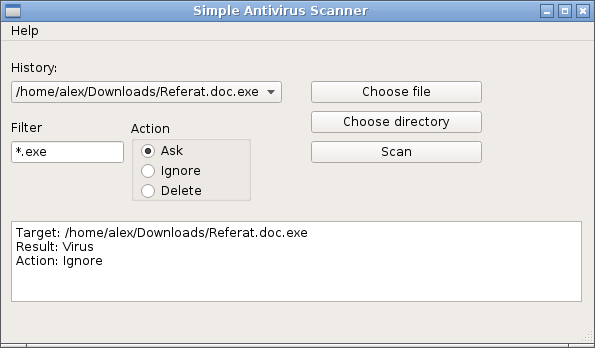
\includegraphics[width=\textwidth]{mainwindow}
\caption{Главное окно программы}
\label{fig:mainwindow}
\end{figure}
\begin{enumerate}
\item При запуске Программа восстанавливает своё состояние на момент последнего
запуска: выбранную пользователем директорию (файл), настройки сканирования,
журнал.
\item В Программе предусмотрен графический диалог выбора директории (файла) для
сканирования.
\item В окне Программы отображается журнал, информирующий Пользователя о работе
Программы. При желании Пользователь может очистить журнал.
\item Программа находит вирусы и поступает с ними так, как указал Пользователь
при запуске сканирования: пропускает, удаляет либо спрашивает Пользователя.
\item Пользователь может указать расширение. В этом случае Программа сканирует
лишь файлы с таким расширением.
\end{enumerate}
\subsection{Нефункциональные требования}
\begin{itemize}
\item Программа не зависает во время выполнения длительных операций
\item Программа занимает не более 512МБ оперативной памяти
\item Для работы Программы не требуются привеллегии суперпользователя, в случае,
если сканируемые файлы доступны для чтения и записи Пользователю.
\end{itemize}
\section{Команда разработки}
Состав команды приведён в таблице \ref{table:team}.
\begin{table}[h]
\centering
\begin{tabular}{|p{25mm}|p{35mm}|l|p{25mm}|}
\hline
ФИО & Роли & Эл. почта & Учётная запись BitBucket \\
\hline
Богданенко А.~О. & Скрам-мастер, техн. писатель, GUI-разработчик
& alexey@bogdanenko.com & abogdanenko \\
\hline
Хамитов К.~Г. & Гл. разработчик & berserq0123@gmail.com & lberserq \\
\hline
\end{tabular}
\caption{Состав команды}
\label{table:team}
\end{table}
Распределение компонентов между разработчиками приведено в Приложении 1.
Подробное распределение обязанностей приведено в Приложении 2.
\section{Типовые сценарии (пользовательские истории)}
\begin{enumerate}
\item Пользователь выбирает директорию (файл) для сканирования. Пользователь
выбирает, что делать с заражёнными файлами. Пользователь запускает сканирование.
Программа сканирует файлы в выбранной директории (выбранный файл), информирует
Пользователя о состоянии работы в журнале. Журнал отображается во время работы
Программы в окне Программы.
\item Пользователь закрыл Программу. Пользователь открыл Программу. Программа
сохранила выбранную пользователем директорию (файл), настройки сканирования,
журнал.
\item Пользователь пожелал очистить журнал, и в окне Программы нашлась для этого
кнопка.
\item Пользователь запустил сканирование директории с 8-гигабайтными HD-видео
файлами. Программа не зависла и не завершилась аварийно.
\item Пользователь запустил сканирование системной директории, на которую у него
нет прав. Программа проинформировала Пользователя на человеческом языке о
проблеме при сканировании.
\item Пользователь указал расширение EXE, Программа сканировала файлы только с
таким расширением.
\end{enumerate}
\section{Экранные формы}
Главное окно программы приведено на рис. \ref{fig:mainwindow}.
\section{Антитребования}
\section{Открытые задачи}
\begin{itemize}
\item Программа запрашивает у Пользователя желаемое действие с заражённым
файлом, и в диалоговом окне есть возможность выполнить это действие для всех
оставшихся файлов.
\item Функция приостановить сканирование
\item Функция отменить сканирование
\end{itemize}
\section{Идеи}
\section{Журнал}
\section{Приложения}
Приложение 1. Компоненты и распределение базовой функциональности сканера за
разработчиками.

Распределение компонентов между разработчиками приведено в таблице
\ref{table:responsibilities}, список классов и функциональность компонентов
приведена в таблице \ref{table:components}.
\begin{table}[h]
\centering
\begin{tabular}{|l|p{3cm}|p{3cm}|}
\hline
Разработчик & Входит в группу / является & Компоненты \\
\hline
Богданенко А. О. & Скрам-мастер & Графический интерфейс, Настройки, Прочее \\
\hline
Хамитов К. Г. & Скрам-команда & Обработчик вредоносных программ, Файловый
браузер, Сигнатурный анализатор, Сканер \\
\hline
\end{tabular}
\caption{Распределение компонентов между разработчиками}
\label{table:responsibilities}
\end{table}

\begin{table}[h]
\centering
\begin{tabular}{|p{25mm}|p{4cm}|l|p{4cm}|}
\hline
Компонент & Классы & Ветвь & Функциональность / предназначение \\
\hline
Графический интерфейс & - & gui & Взаимодействие с пользователем \\
\hline
Настройки & - & settings & Сохранение, загрузка настроек \\
\hline
Прочее & GeneralException & miscellaneous
& Генерация исключений в пределах проекта \\
\hline
Обработчик вредоносных программ
& MalwareInfo, MalwareHandlerPolicy, MalwareHandler
& malware\_handler & Действия над вредоносными файлами \\
\hline
Файловый браузер & FileInfo, FileBrowser & file\_browser
& Поиск файлов и директорий \\
\hline
Сигнатурный анализатор & SignatureAnalyzer & signature\_analyzer
& Загрузка базы сигнатур из файла, поиск информации о файле в БД \\
\hline
Сканер & Scanner & scanner & Обеспечение доступа к остальным возможностям \\
\hline
\end{tabular}
\caption{Список классов и функциональность компонентов}
\label{table:components}
\end{table}
